%%%%%%%%%%%%%%%%%%%%%%%%%%%%%%%%%%%%%%%%%%%%%%%%%%%%%%%%%%%%%%%%%%%%%%%%%%%%%%%%
% results.tex:  
%%%%%%%%%%%%%%%%%%%%%%%%%%%%%%%%%%%%%%%%%%%%%%%%%%%%%%%%%%%%%%%%%%%%%%%%%%%%%%%%
\chapter{Results}
\label{results}

The events in the partial disappearance region and the tag/probe invariant mass distribution for events in the complete disappearance region are shown in \Cref{fig:invMassResult} for the expected data and estimated backgrounds.

\begin{figure}[htbp]
	\centering
	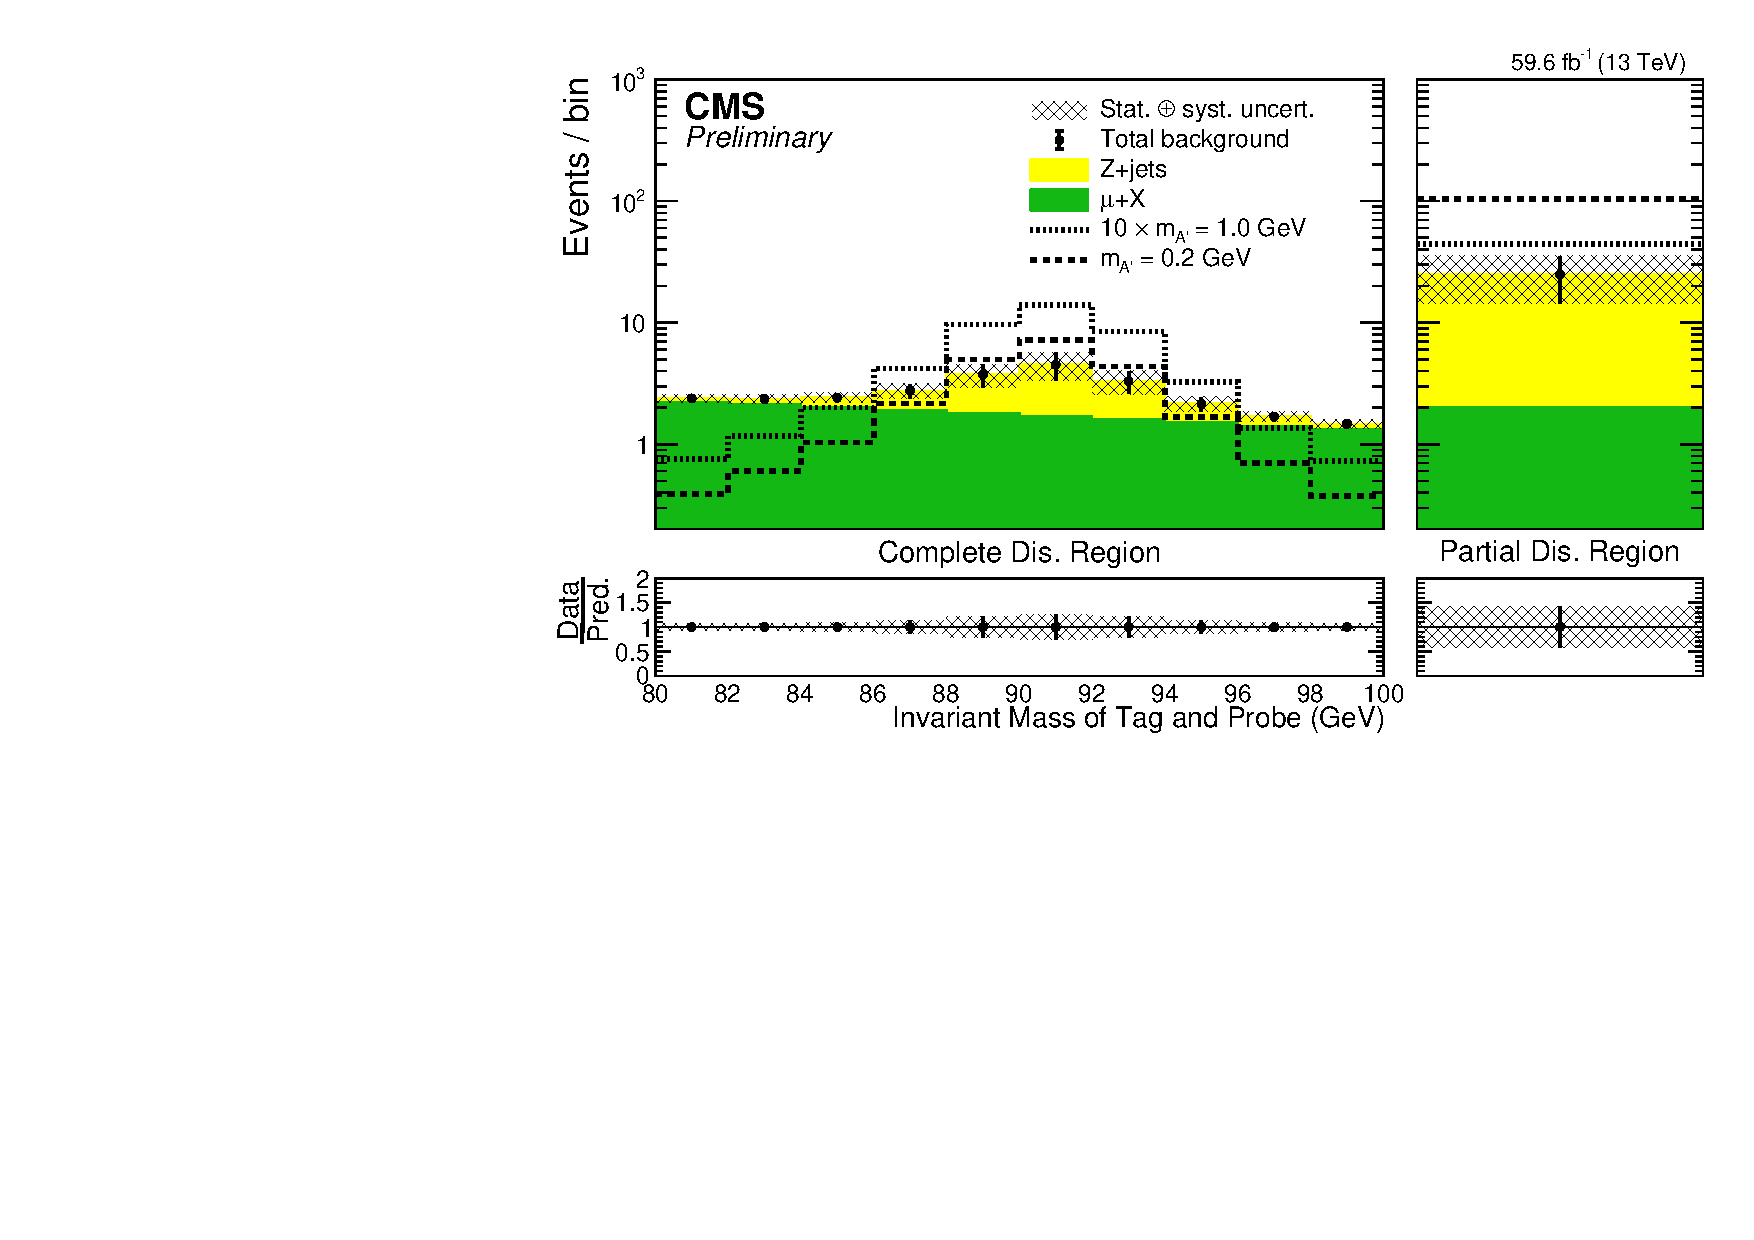
\includegraphics[width=0.8\textwidth]{figures/bdtScore_partialDisappearanceBDT_0p2.pdf}
	\caption[Observed Signal Region Events]{The di-muon invariant mass of complete disappearance events and the number of partial disappearance events seen in data, as well as the predicted backgrounds from simulation and the off-peak control region.}
	\label{fig:invMassResult}
\end{figure}

The results are combined with the measured fixed target luminosities from the signal simulation in order to interpret them as limits on the square of the mixing paramer, which the \dbrem interaction rate is directly proportional to.
The expected upper limits are presented in \Cref{fig:limits} as a function of the dark photon mass. 

\begin{figure}[htbp]
	\centering
	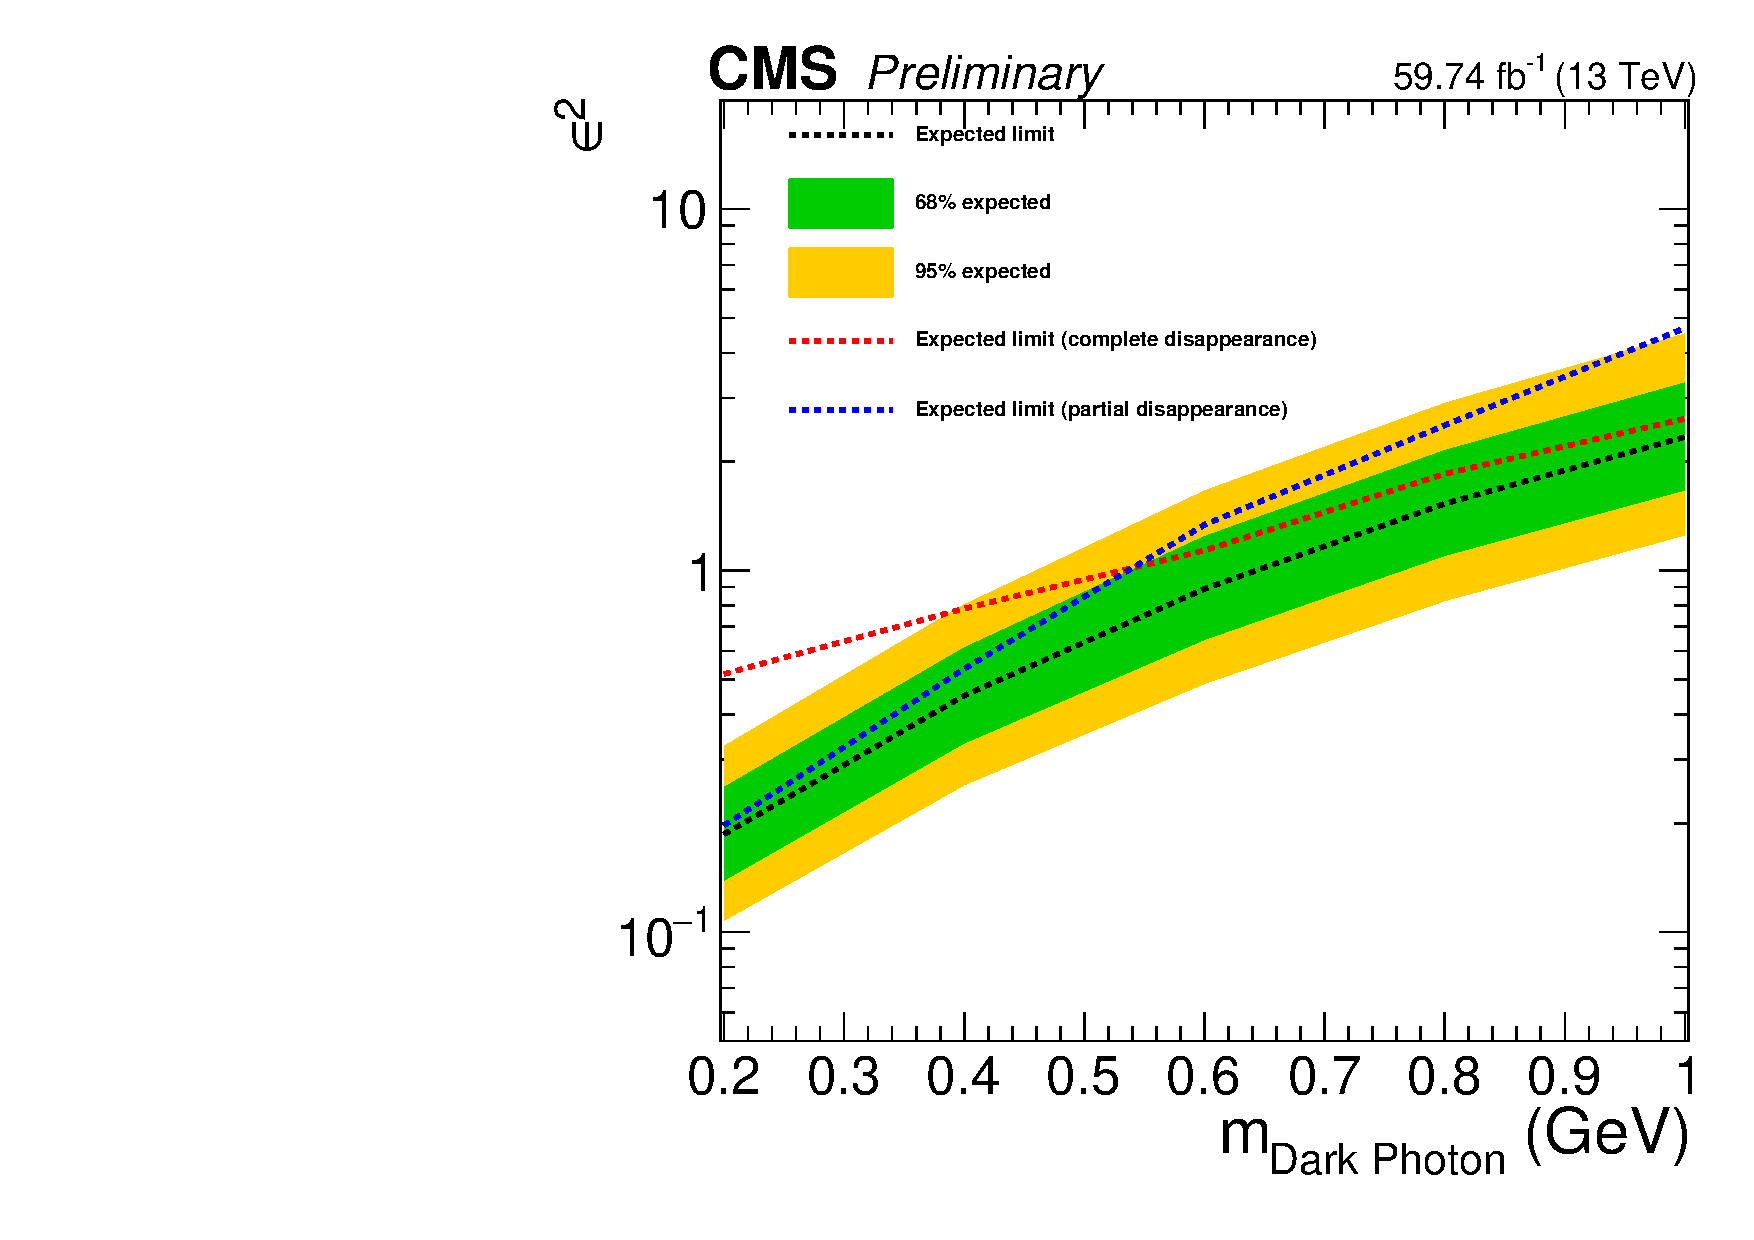
\includegraphics[width=0.8\textwidth]{figures/Limit_AllRegions.pdf}
	\caption[Exclusion Limits on the Dark Photon Mixing Parameter]{The exclusion limit for the square of the dark photon mixing parameter as a function of the A' mass.}
	\label{fig:limits}
\end{figure}

At lower masses the partial disappearance region dominates, as the lighter mass dark photons tend to have higher energy outgoing muons, while the complete disappearance region has more significance for larger A' masses. 
The decreasing cross section with dark photon mass decreases the interaction rate more quickly than the relative increase in selection efficiency created by the lower energy outgoing muons at large A' mass, resulting in overall lower exclusion limits on $\epsilon^{2}$ at small mediator masses. 

Distributions of variables used for signal selection are predicted by using MC for DY backgrounds and re-scaling events from the off-peak control region for $\mu$+X backgrounds.
For the complete disappearance region, the expected HCAL and ECAL isolations are shown in \Cref{fig:totHcalIso}, the distance from the probe track to the nearest CSC segment and the nearest standalone muon are shown in \Cref{fig:totCSCStaDr}, and the number of HE hits along the probe track is shown in \Cref{fig:totHitsOverThresh}.

\begin{figure}[htbp]
	\centering
	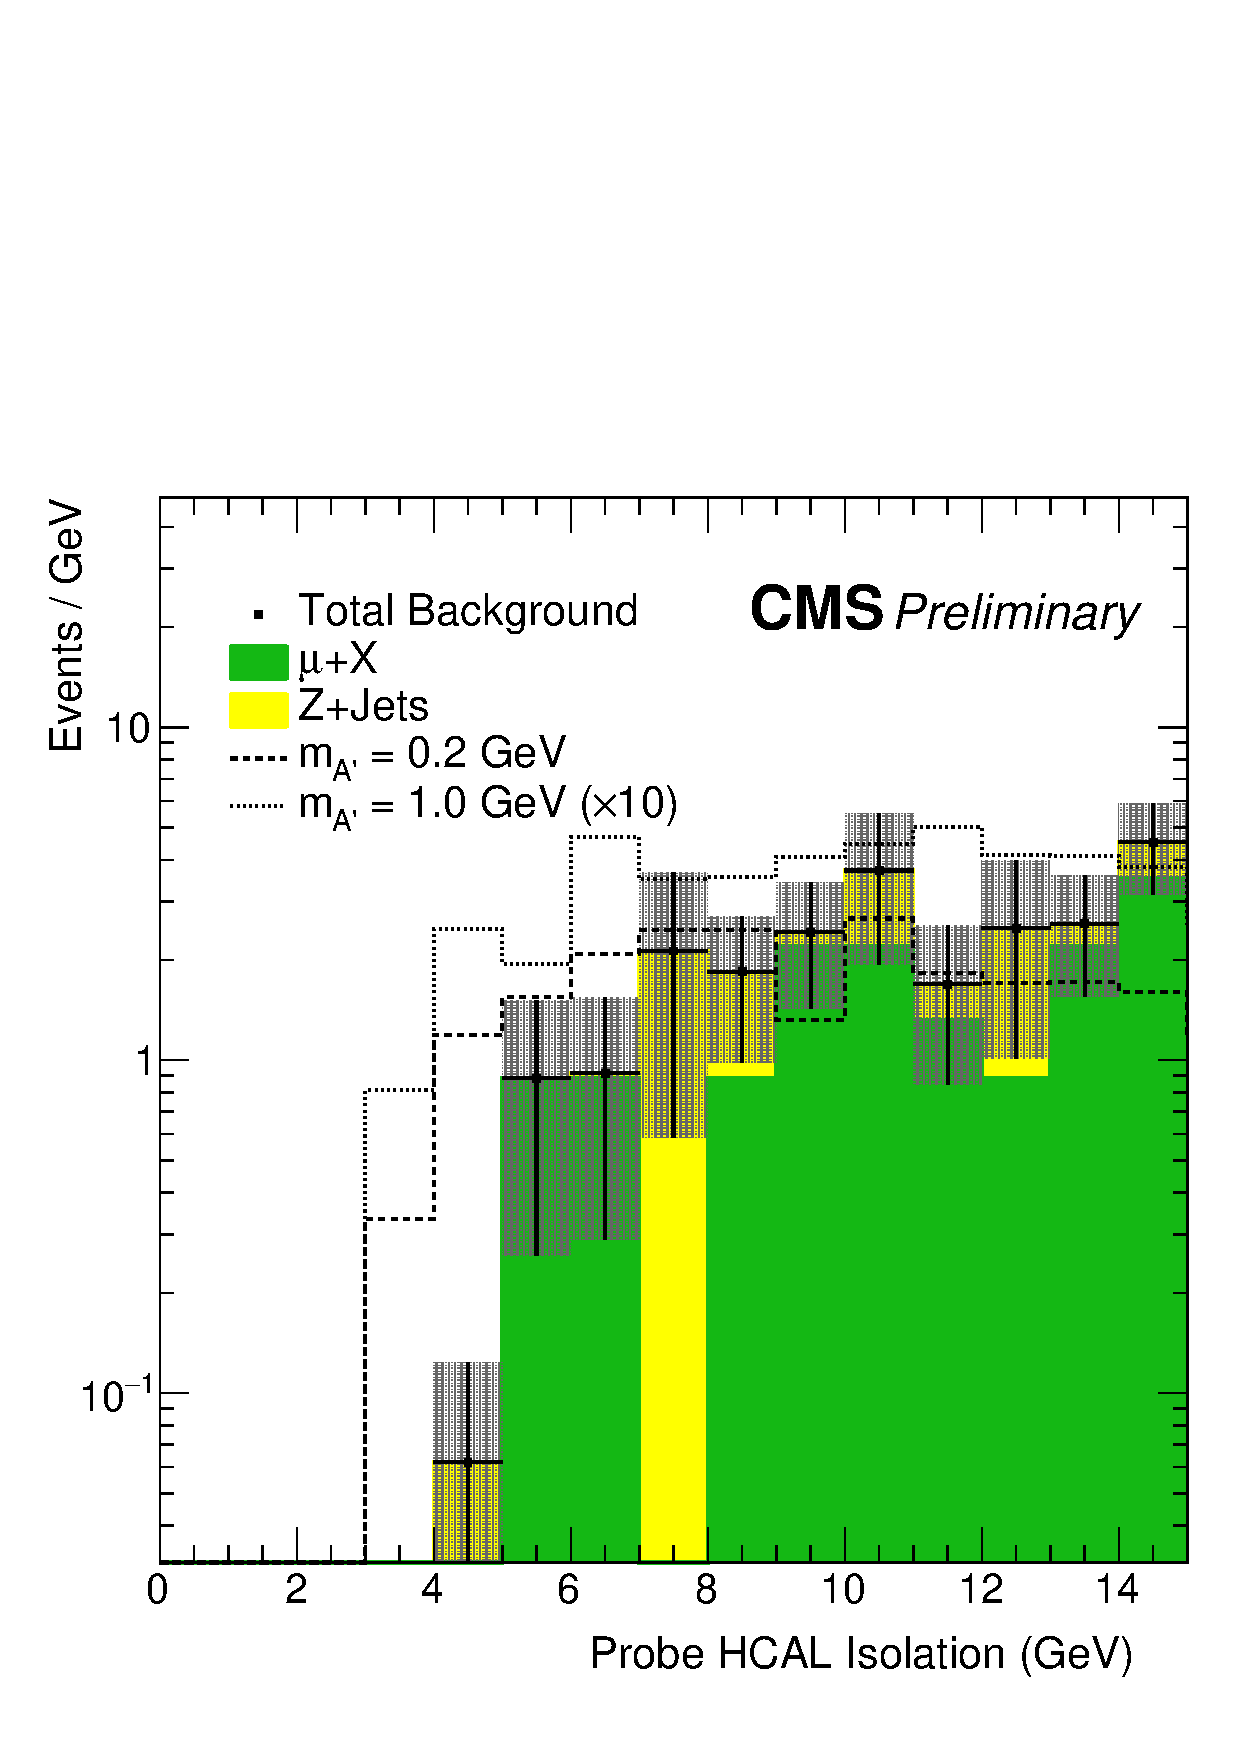
\includegraphics[width=0.45\textwidth]{figures/totDisappHcalIso.pdf}
	\hspace{0.01\textwidth}
	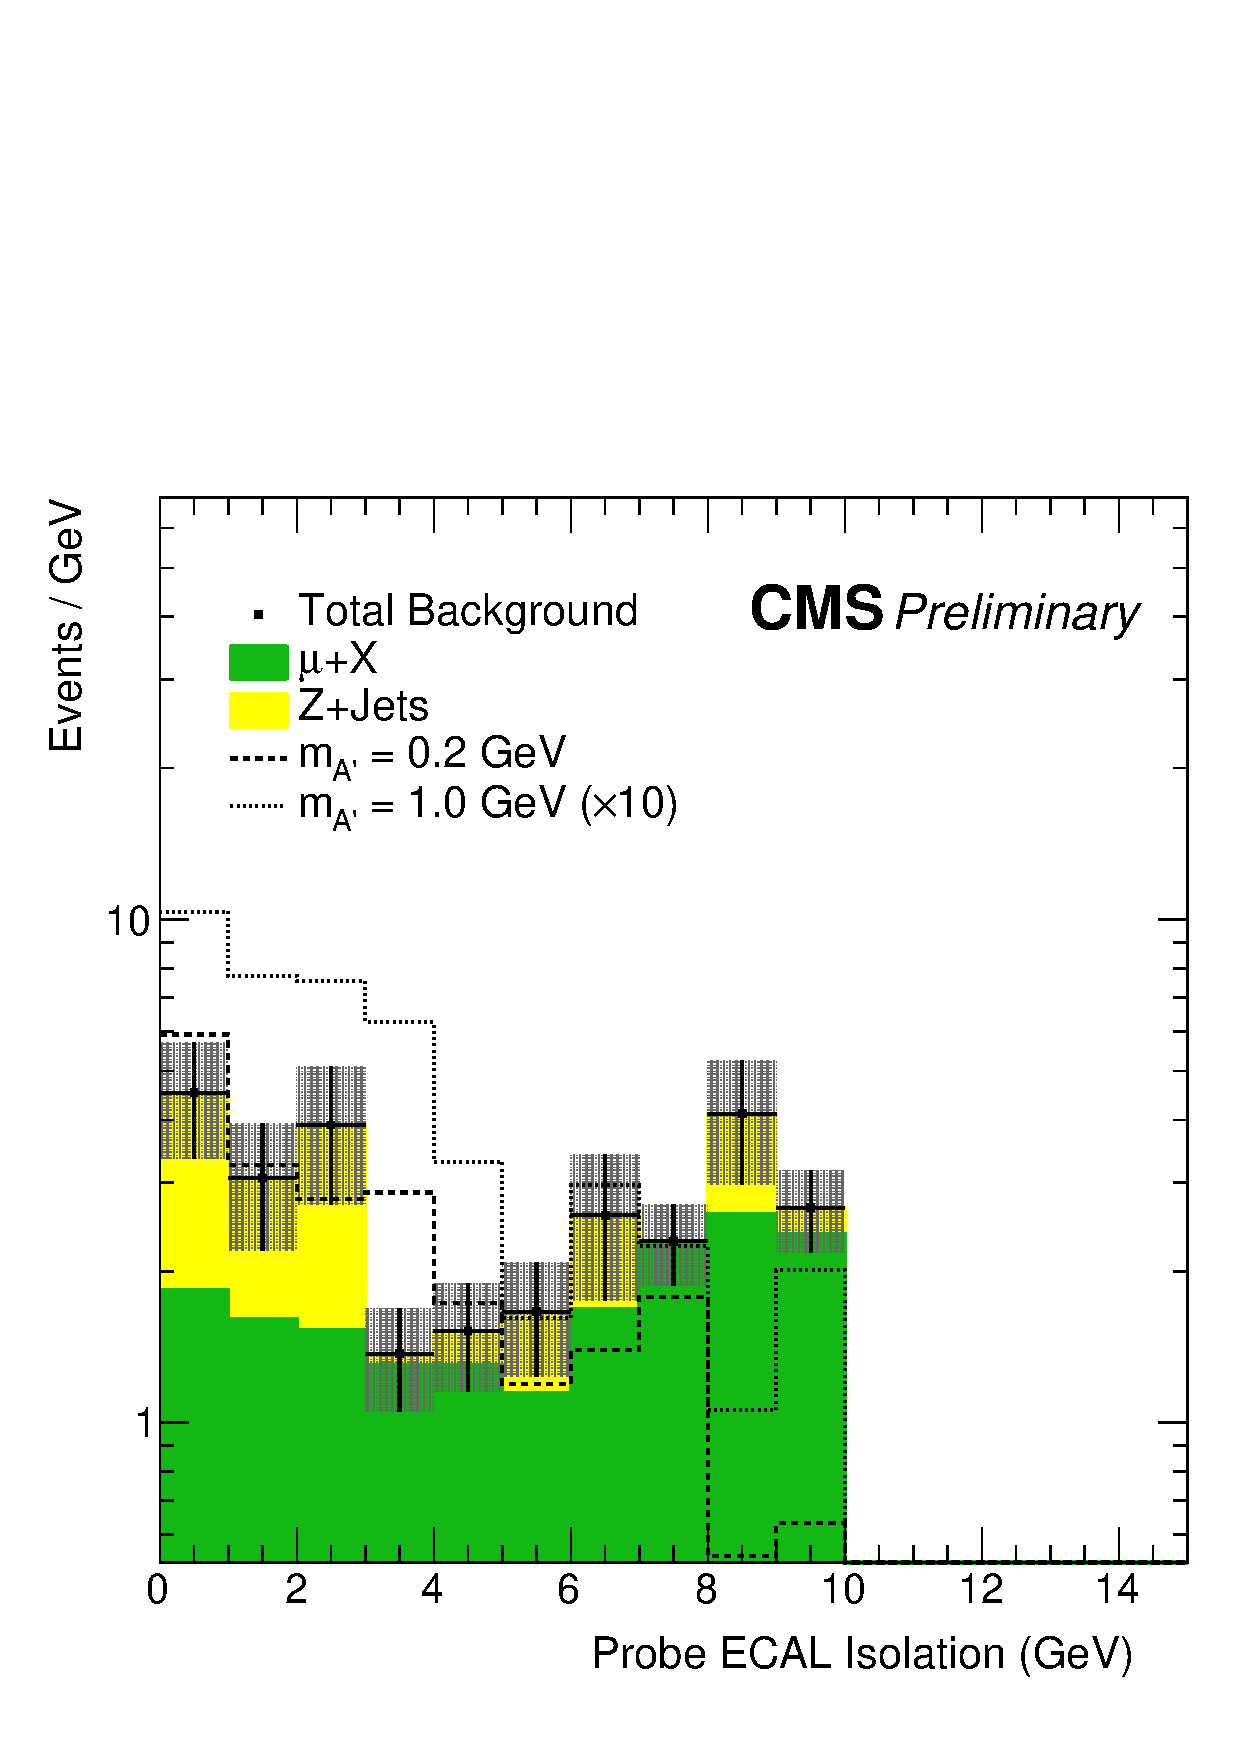
\includegraphics[width=0.45\textwidth]{figures/totDisappEcalIso.pdf}
	\caption[Expected Complete Disappearance Isolation]{The expected distributions of HCAL (left) and ECAL (right) isolation for the complete disappearance region. Signal events tend to have lower isolation in both the ECAL and HCAL, as $\mu$+X events frequently occur in particle showers and DY events have visible energy deposits from SM bremsstrahlung.}
	\label{fig:totHcalIso}
\end{figure}

\begin{figure}[htbp]
	\centering
	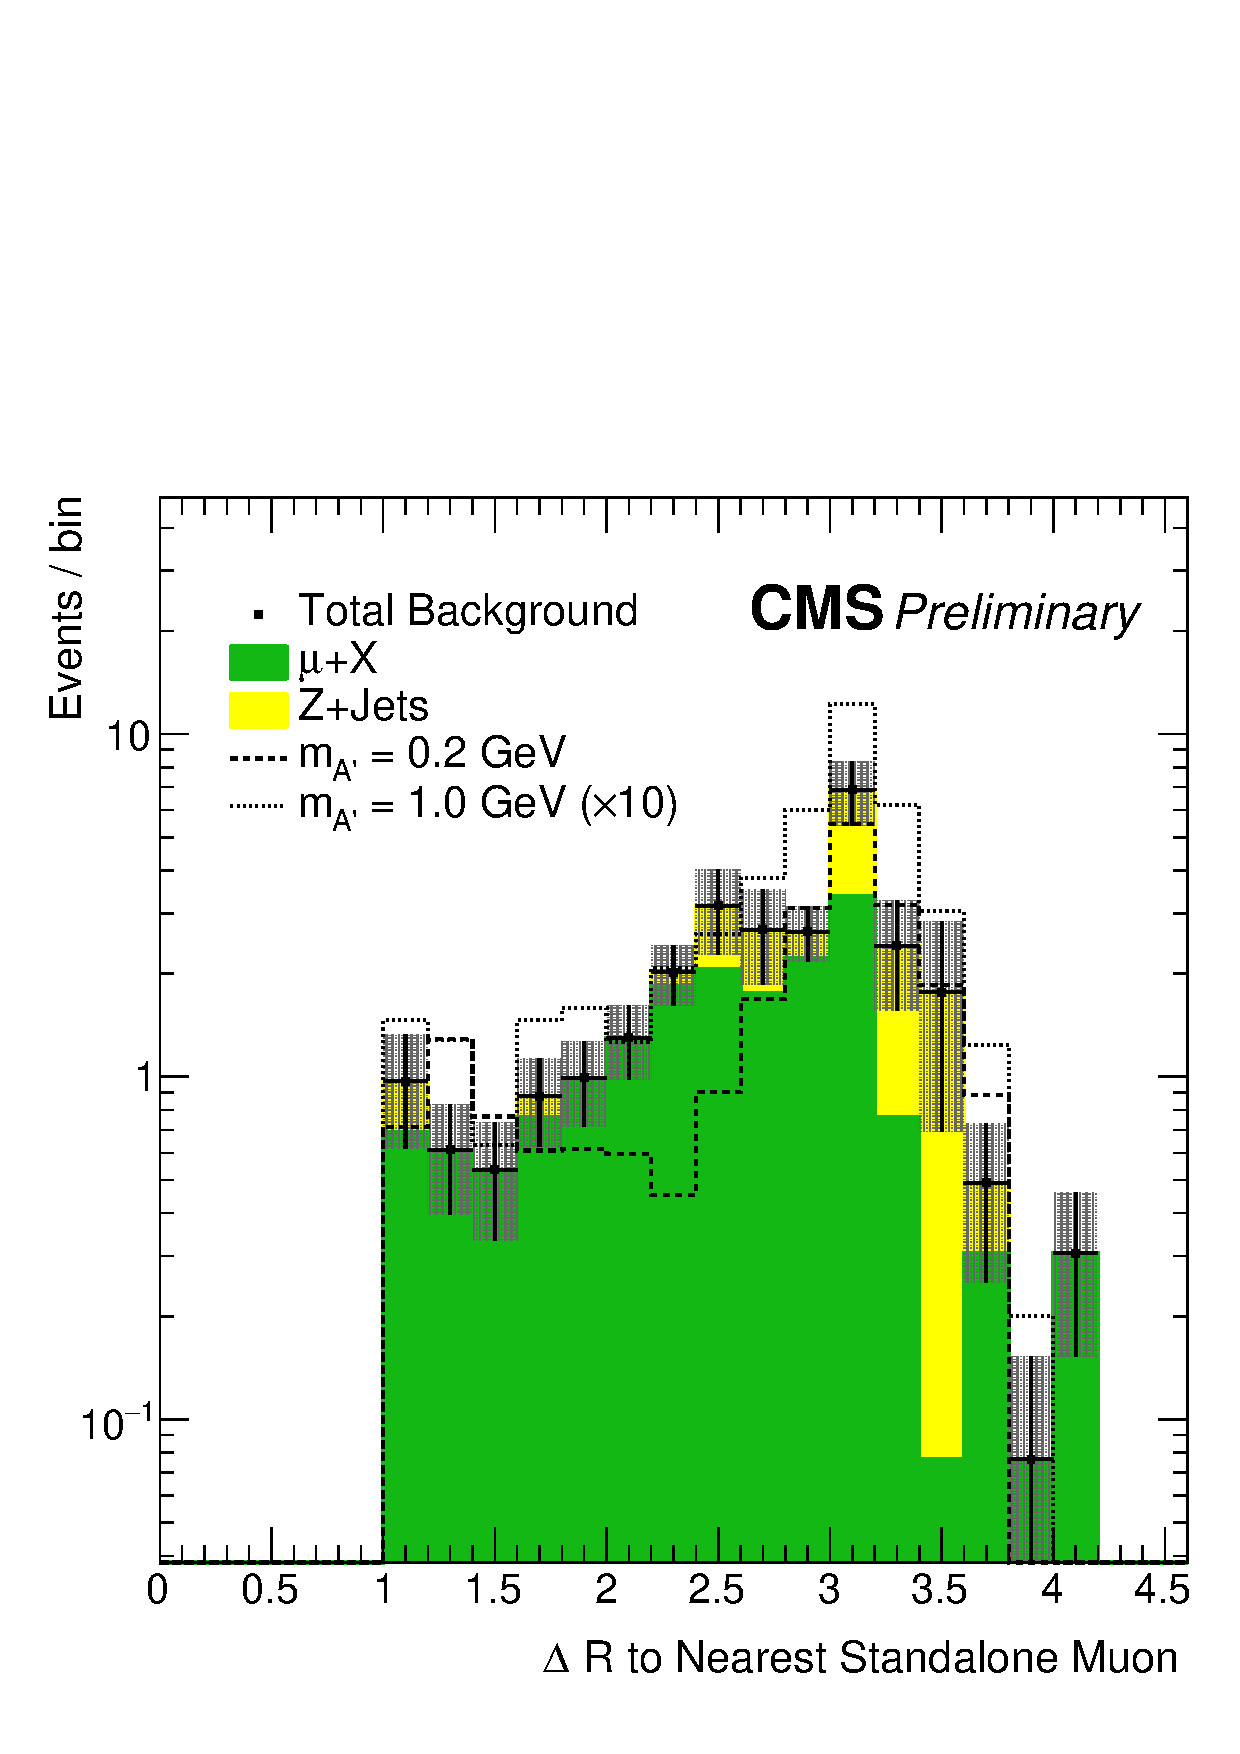
\includegraphics[width=0.45\textwidth]{figures/totDisappStaDr.pdf}
	\hspace{0.01\textwidth}
	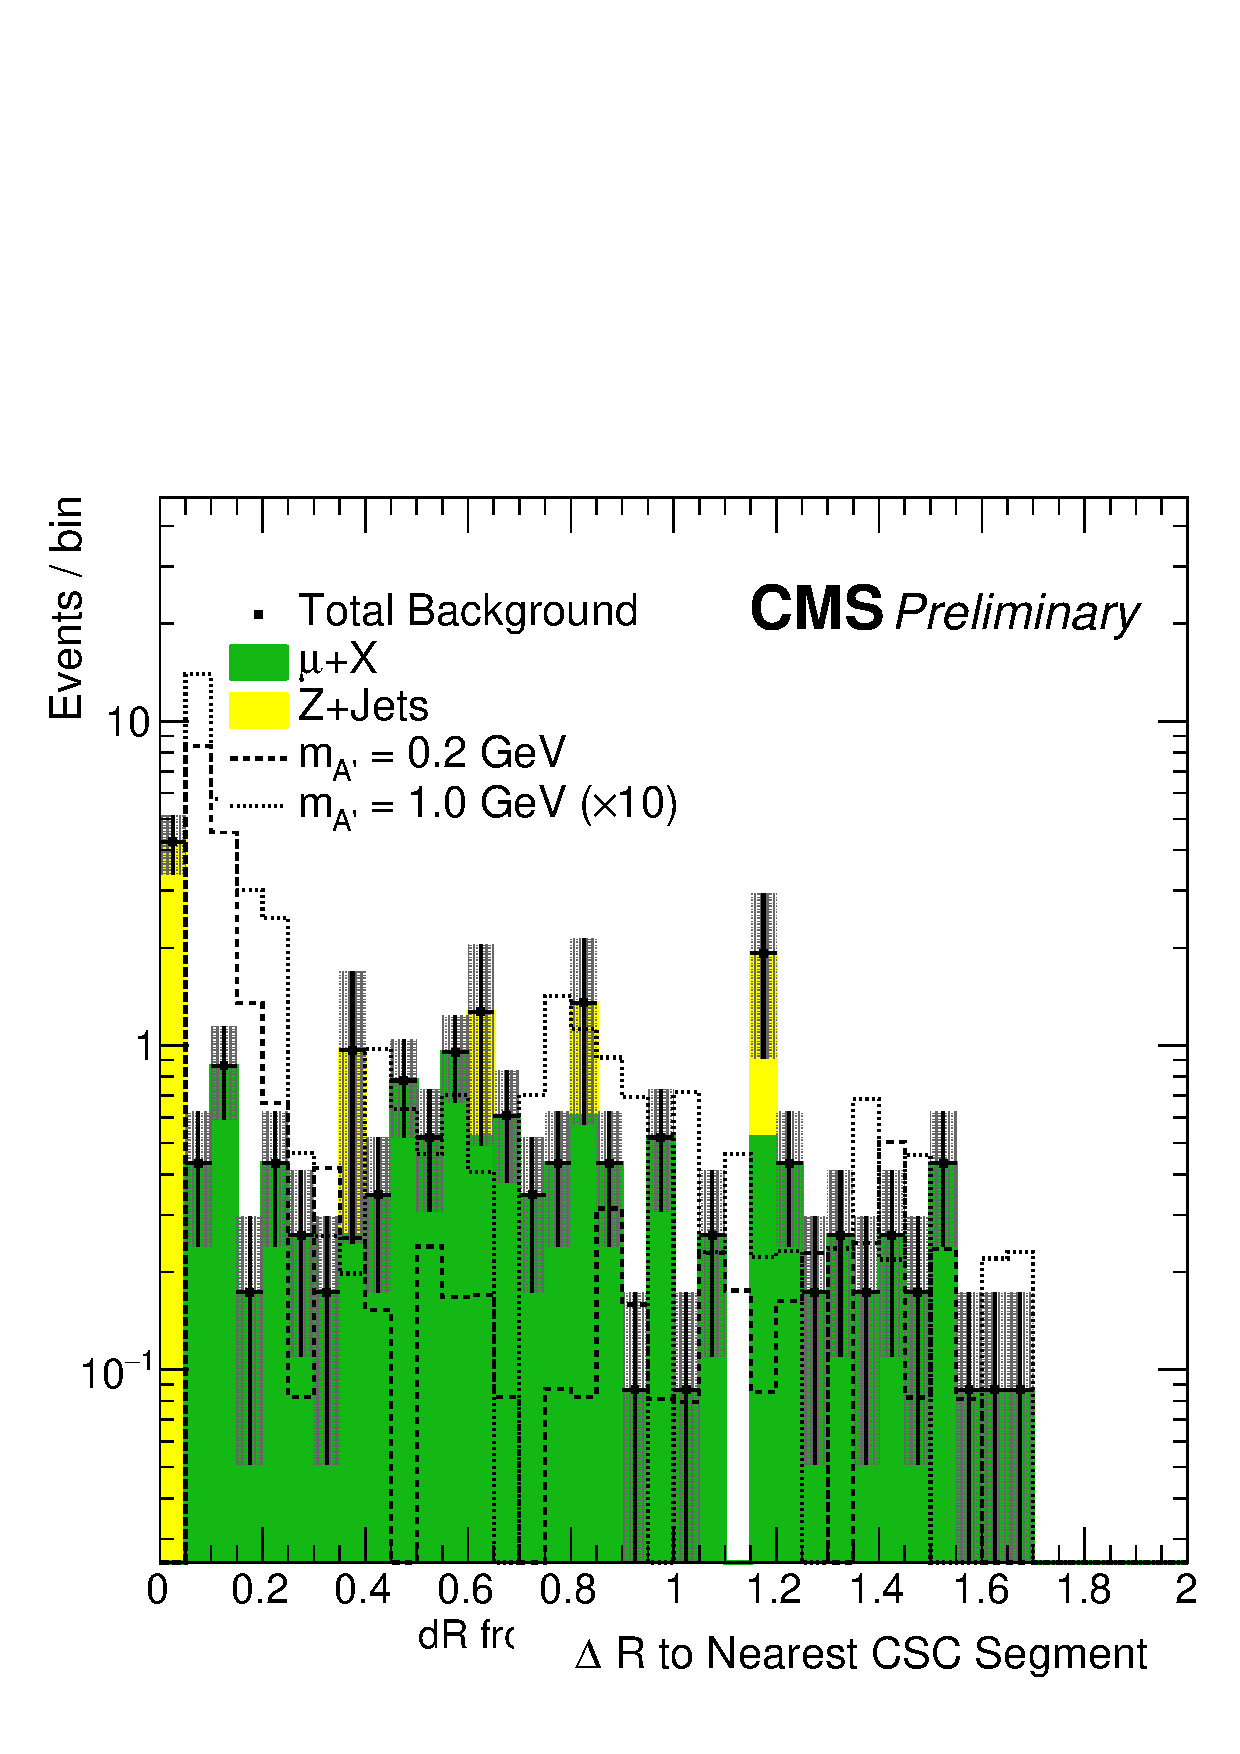
\includegraphics[width=0.45\textwidth]{figures/totDisappCscDr.pdf}
	\caption[Expected Complete Disappearance Muon Chamber Features]{The expected distance to the nearest standalone muon (left) and nearest CSC segment (right) for the complete disappearance region. The DY events below 0.1 originate from the CSC efficiency correction applied, where events with only one nearby CSC segment are counted as having zero to correct for inefficiencies in the detector (see \Cref{sec:missedMuons}).}
	\label{fig:totCSCStaDr}
\end{figure}

\begin{figure}[htbp]
	\centering
	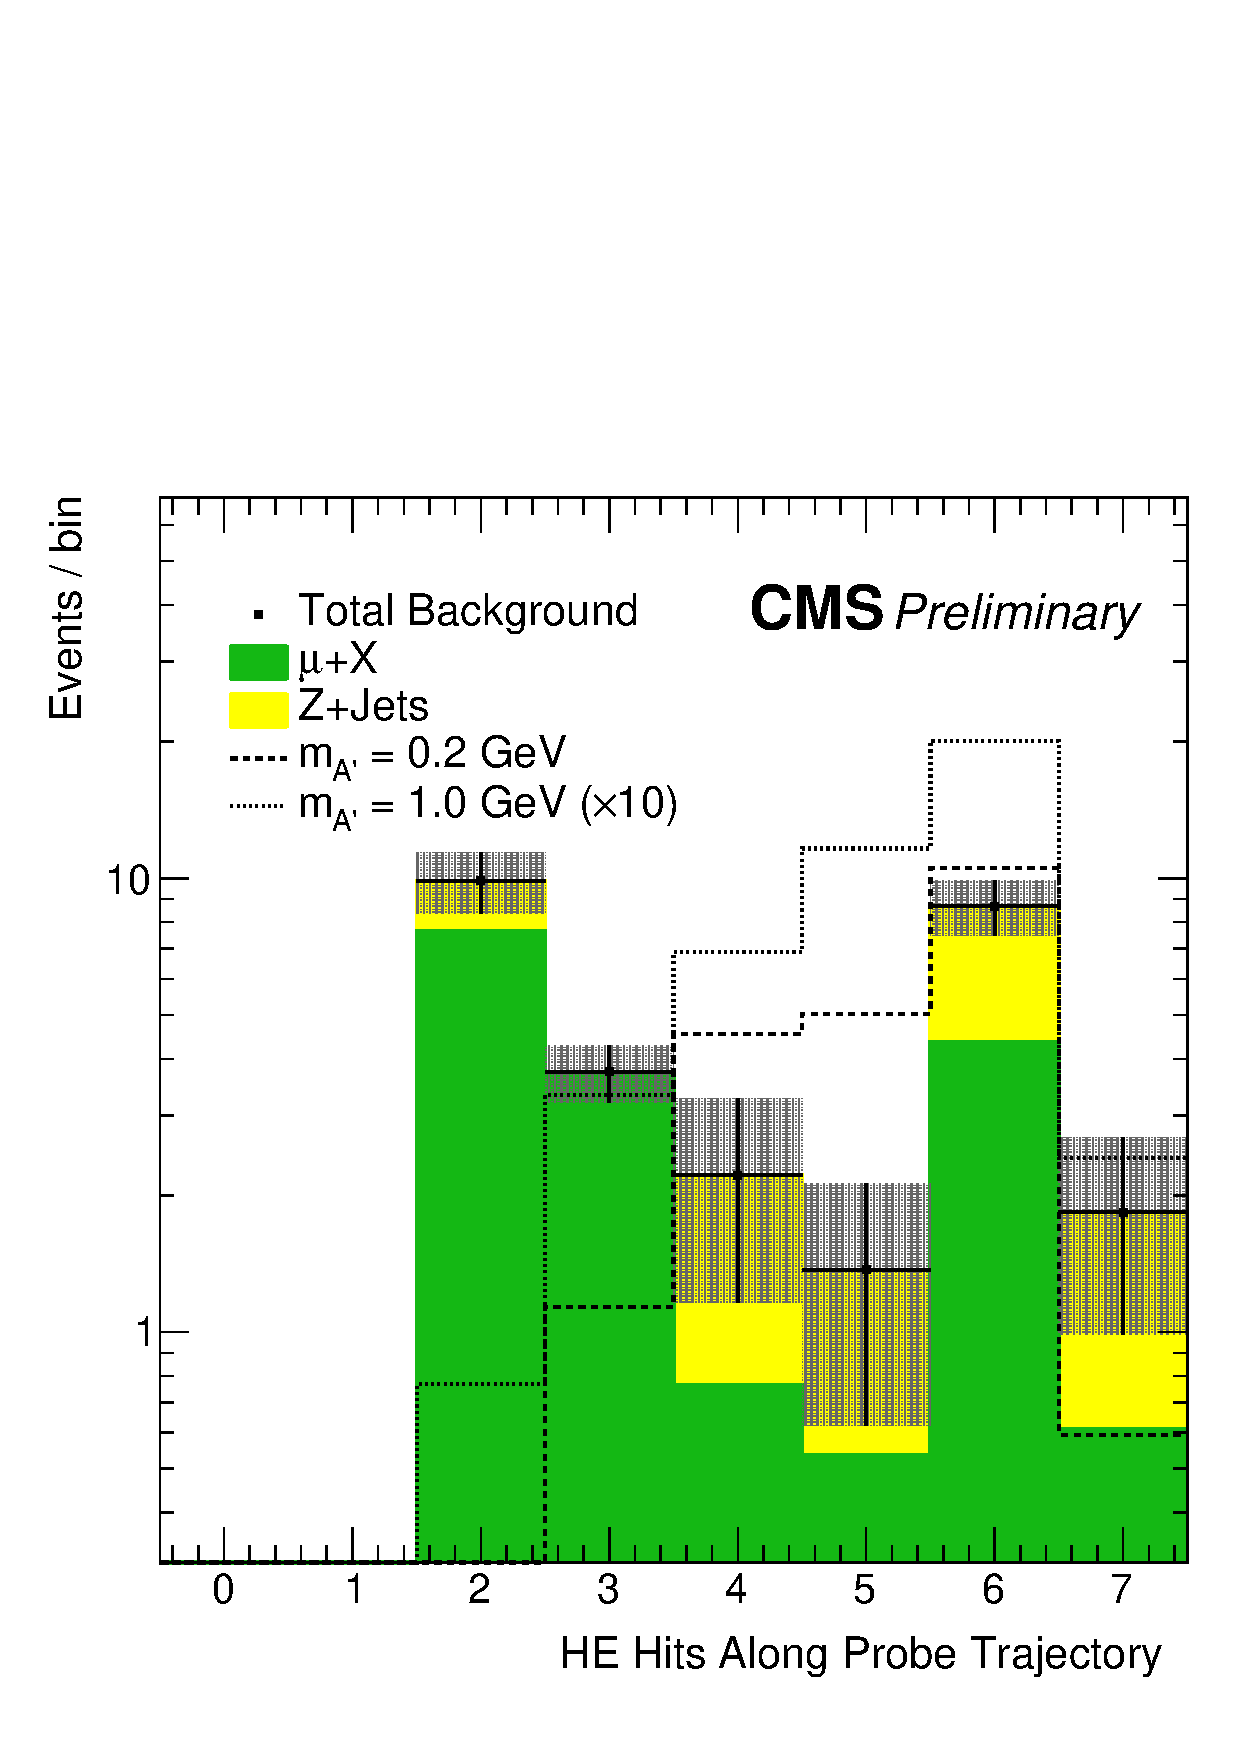
\includegraphics[width=0.45\textwidth]{figures/totDisappHitsOverThresh.pdf}
	\caption[Expected Complete Disappearance HE Hits]{The expected number of HE hits along the probe track trajectory in the complete disappearance region. $\mu$+X backgrounds tend to have fewer HE hits as non-muon backgrounds are absorbed before traversing the full HCAL, while signal events frequently have several missing hits due to being stopped after \dbrem.}
	\label{fig:totHitsOverThresh}
\end{figure}

For the partial disappearance region, the distributions of standalone muon $\Delta$E/E, standalone muon $\Delta$R, CSC $\Delta$R in station one, HE energy in depth four, standalone muon $\chi^{2}$, and standalone muon $\Delta\phi$ are shown in \Cref{fig:partSta,fig:partStat,fig:partStaFeat} for events with BDT scores $>$0.98.
DY events form by far the largest background process in this region, and so only DY MC and signal MC are included.

\begin{figure}[htbp]
	\centering
	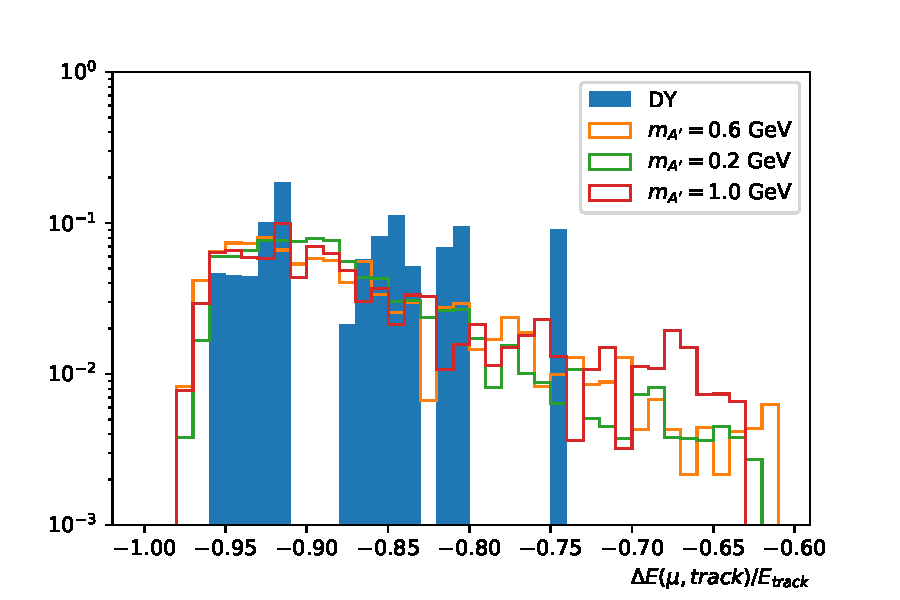
\includegraphics[width=0.45\textwidth]{figures/partDisStaDE.pdf}
	\hspace{0.01\textwidth}
	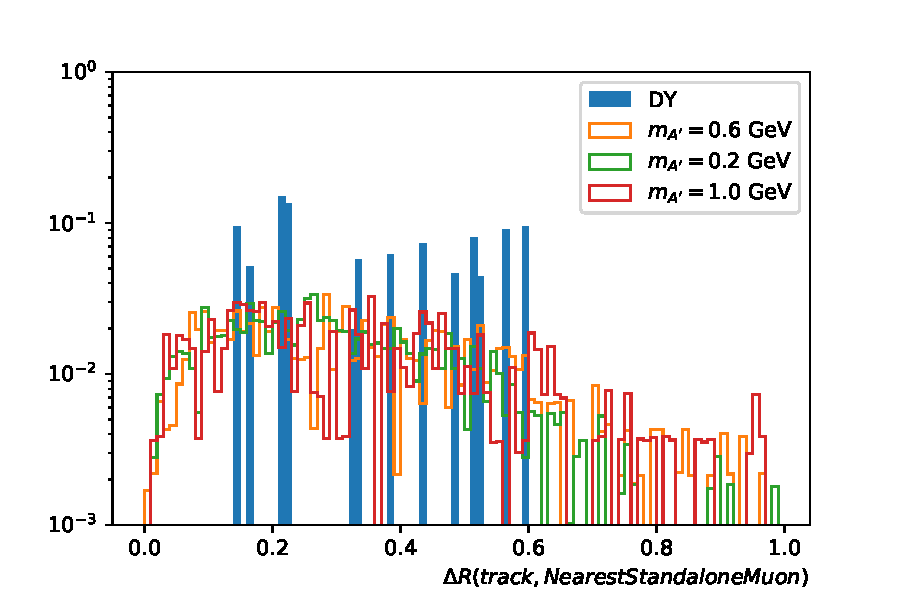
\includegraphics[width=0.45\textwidth]{figures/partDisStaDr.pdf}
	\caption[Expected Partial Disappearance Standalone Muon Features]{The distributions of the fractional difference between the standalone muon energy and the probe track energy and the $\Delta$R to the nearest standalone muon for events with BDT scores $>$0.98.}
	\label{fig:partSta}
\end{figure}

\begin{figure}[htbp]
	\centering
	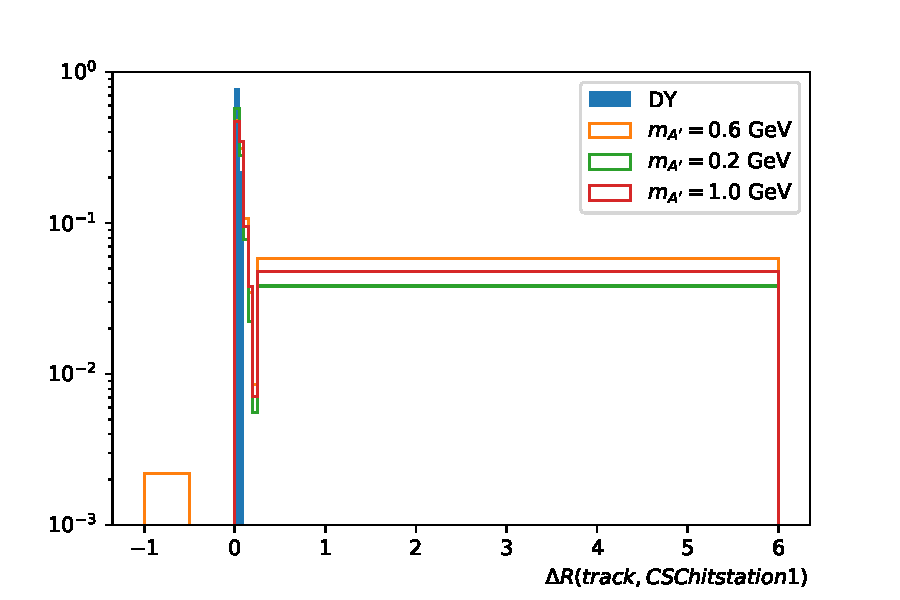
\includegraphics[width=0.45\textwidth]{figures/partDisCSCdr_one.pdf}
	\hspace{0.01\textwidth}
	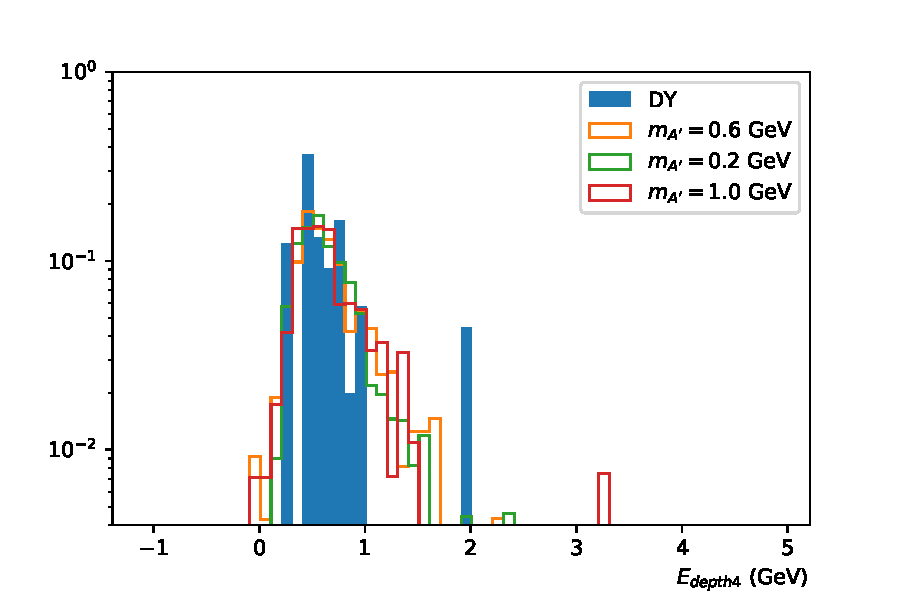
\includegraphics[width=0.45\textwidth]{figures/partDisHCALE_four.pdf}
	\caption[Expected Partial Disappearance CSC and HCAL Features]{The distance to the nearest muon segment in the first CSC station and the HCAL energy in the fourth HE depth. Station one and depth four have the highest feature importance of the CSC stations and HE depths, respectively.}
	\label{fig:partStat}
\end{figure}

\begin{figure}[htbp]
	\centering
	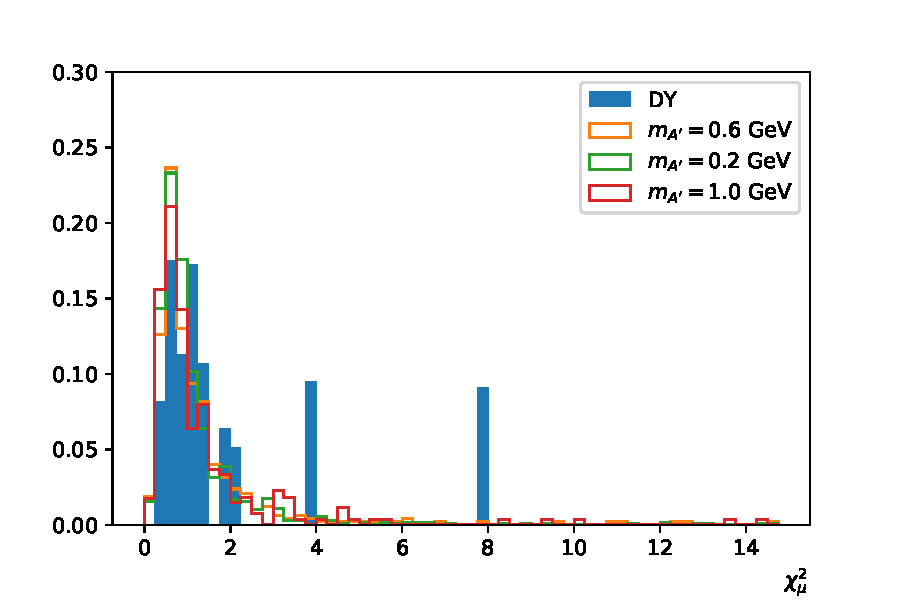
\includegraphics[width=0.45\textwidth]{figures/partDisStaChi.pdf}
	\hspace{0.01\textwidth}
	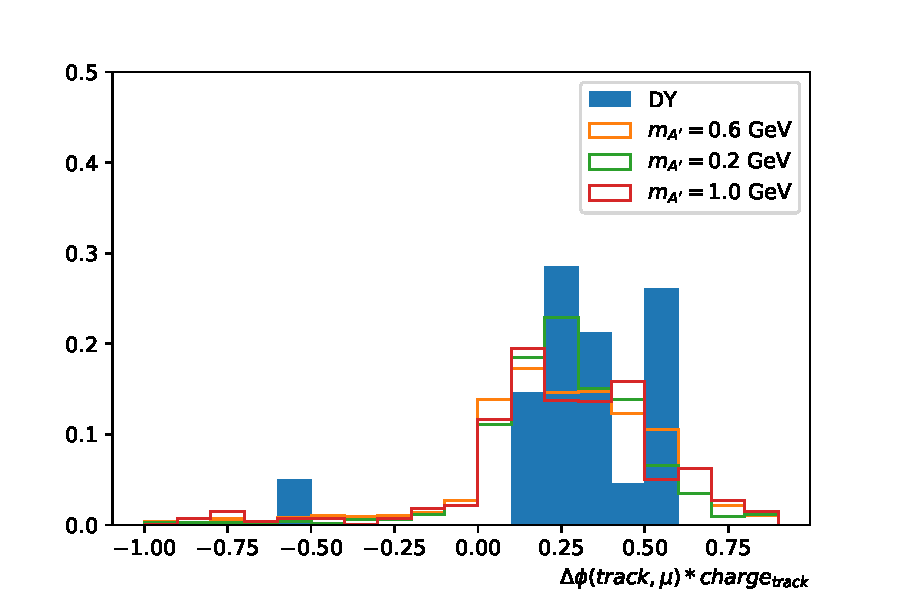
\includegraphics[width=0.45\textwidth]{figures/partDisStaPhi.pdf}
	\caption[Expected Partial Disappearance Standalone Muon Quality]{The reduced $\chi^{2}$ and the $\Delta\phi$ between the probe track and standalone muon multiplied by the probe charge for partial disappearance events with BDT scores $>$0.98.}
	\label{fig:partStaFeat}
\end{figure}
